\chapter{力、相空间与守恒定律}

\lectureoverview{运动定律不能仅仅把熟悉的物理量联系起来。它必须指定系统的状态，把该状态从一个时刻带到下一个时刻，并揭示哪些区分和哪些量在运动中得以保留。我们将先检验一条看似合理但错误的力定律，然后把状态从位置扩展到相空间，最后导出动量守恒和能量守恒，由此到达牛顿力学。}

\section{一条有用的错误定律}

日常运动由摩擦主导。把一个重物在地板上推一下，它就会移动；停止推，它很快就停下来。推得越用力，速度通常越大；而越重的物体需要越大的推力。在这样的世界里，人们自然会设想力本身产生速度。这就是亚里士多德对运动的描述背后的基本直觉。

滑冰提供了缺失的经验。滑冰者需要力来启动、停止或改变方向，但一旦处于运动之中，继续滑行并不需要力。假如亚里士多德研究的是近乎无摩擦的冰面而不是普通地面，那么力--速度这一直觉中的缺陷就会难以被忽略得多。

为了揭示这一直觉错在哪里，让我们给它一个精确的现代形式。我们写下这条故意不正确的方程

\begin{equation}
  \mathbf F=m\mathbf v.
  \label{eq:aristotle-vector-law}
\end{equation}

这不是牛顿定律，不应作为物理内容来记忆。它的价值在于诊断：一旦一条文字规则变成了方程，我们就可以追问它是否预言运动，以及它是否保留了足够的信息以重建过去。课堂上关于希腊语中表示力的词的那段简短讨论指向\emph{dynamis}，dynamo 和 dynamics 等词也源自同一词根，但术语相对于对定律本身的检验来说是次要的。

\begin{figure}[htbp]
  \centering
  \includegraphics[width=0.82\textwidth]{lecture_02_figure_02.png}
  \caption{用来检验可预言性和可逆性的、故意错误的力--速度定律。}
  \lectureframe{00:04:51}
\end{figure}

把运动限制在一个空间坐标上。由于\(v=\dot x\)，该定律为

\begin{equation}
  F(t)=m\dot x(t).
  \label{eq:aristotle-1d}
\end{equation}

现在把时间分成长度为\(\delta\)的短区间。在一个区间内，

\begin{equation}
  \dot x(t)\simeq
  \frac{x(t+\delta)-x(t)}{\delta}.
  \label{eq:first-difference}
\end{equation}

代入式~\eqref{eq:aristotle-1d}得到

\begin{equation}
  x(t+\delta)
  =x(t)+\frac{\delta}{m}F(t).
  \label{eq:aristotle-update}
\end{equation}

这具有真正的更新规则的形式。如果当前的位置和力已知，那么下一个频闪时刻的位置就随之确定。然而，当力为零时，亚里士多德的规则给出\(\dot x=0\)：物体必须保持静止。没有维持力就没有运动，这一点从一开始就被排除在外。

\begin{figure}[htbp]
  \centering
  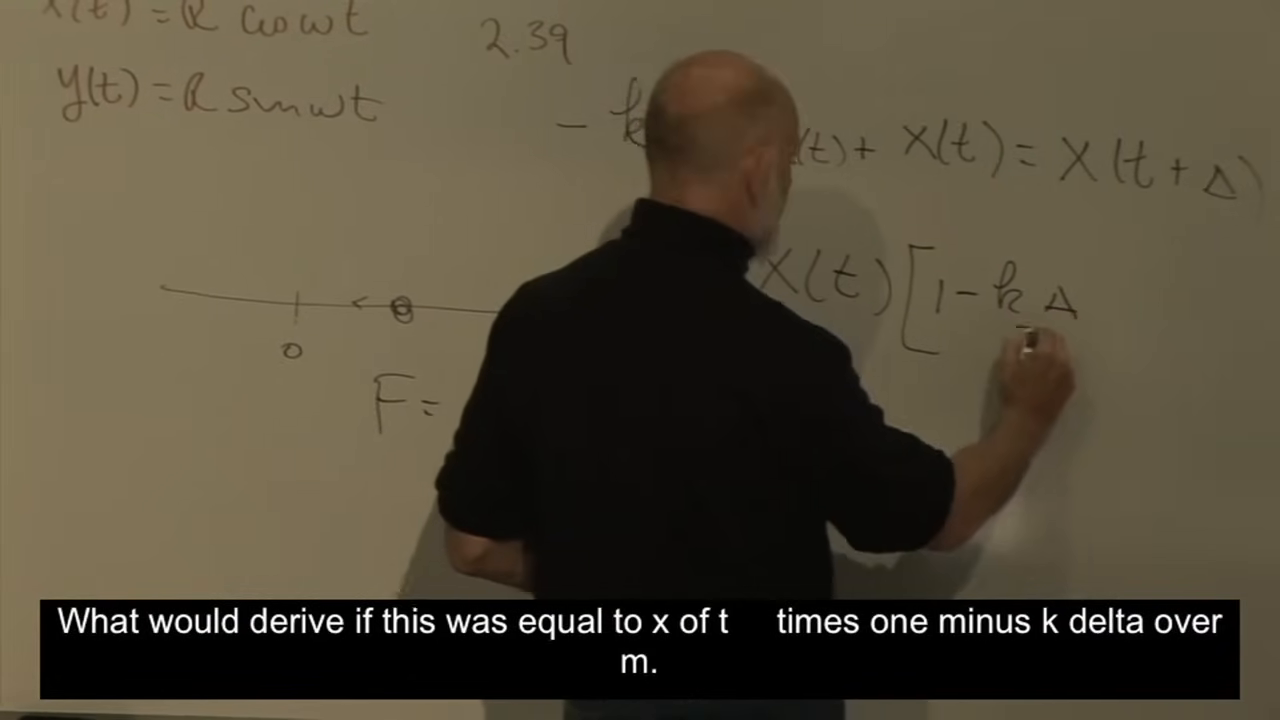
\includegraphics[width=0.84\textwidth]{lecture_02_figure_07.png}
  \caption{带恢复力的离散亚里士多德更新。每一步都把位移乘以一个略小于一的因子。}
  \lectureframe{00:10:15}
\end{figure}

\subsection{亚里士多德力学中的弹簧}

考虑一个连接在弹簧上的粒子，平衡位置在\(x=0\)。位移产生恢复力

\begin{equation}
  F(x)=-kx,
  \qquad k>0.
  \label{eq:hooke-law}
\end{equation}

把这个力代入式~\eqref{eq:aristotle-update}得到

\begin{equation}
  x(t+\delta)
  =\left(1-\frac{k\delta}{m}\right)x(t).
  \label{eq:aristotle-spring-update}
\end{equation}

对于足够小的\(\delta\)，括号中的因子略小于一。因此每一次更新都按同一比例减小位移：

\begin{equation}
  x_n=\left(1-\frac{k\delta}{m}\right)^n x_0.
  \label{eq:aristotle-geometric-decay}
\end{equation}

连续方程及其解为

\begin{align}
  m\dot x&=-kx,
  \label{eq:aristotle-spring-continuous}\\
  x(t)&=x(0)e^{-kt/m}.
  \label{eq:aristotle-spring-solution}
\end{align}

弹簧并不振荡。从任意位移释放，它都指数式地趋近原点，越靠近原点运动得越慢。

\begin{figure}[htbp]
  \centering
  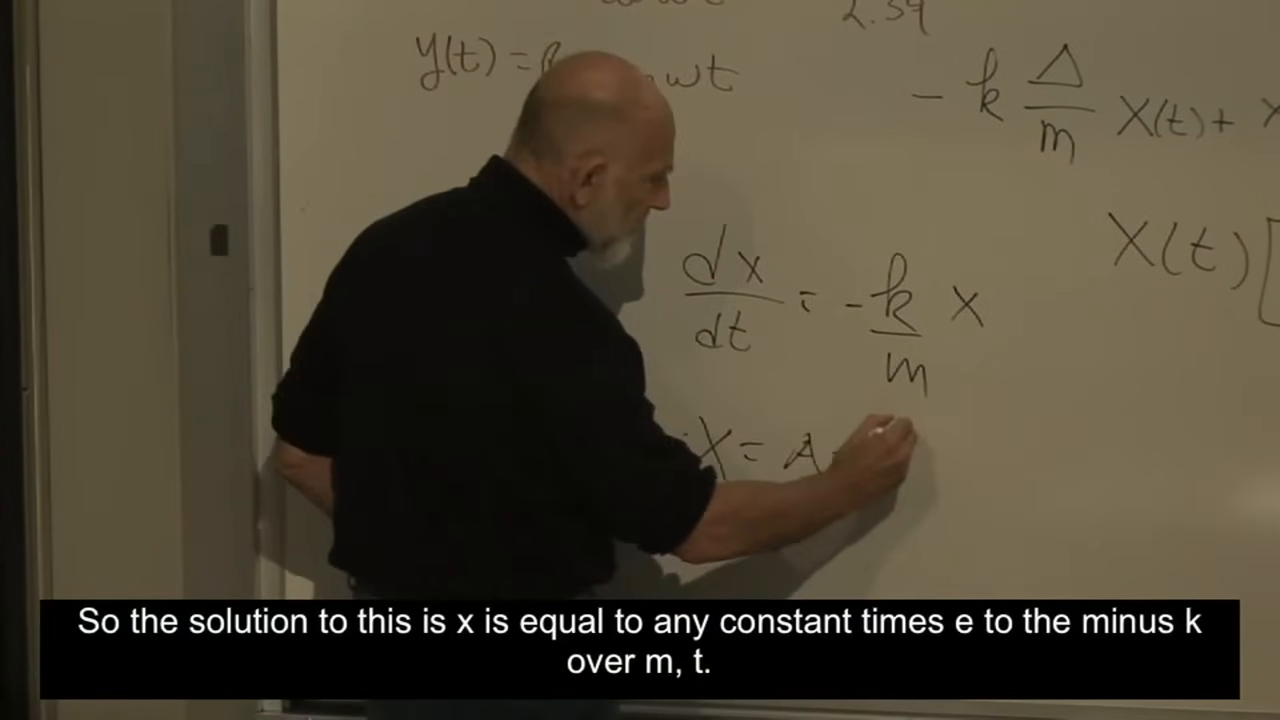
\includegraphics[width=0.84\textwidth]{lecture_02_figure_08.png}
  \caption{亚里士多德弹簧方程的指数解。位移衰减而不是振荡。}
  \lectureframe{00:12:02}
\end{figure}

未来很容易预言：每一个初始位移都趋近同一个静止构型。过去则是另一回事。假设在原点附近以有限的精度观测该粒子。它可能从许多不同的位移中的任意一个开始，因为所有这些位移的指数式微小残余最终都落在同一测量容差之内。在完美的数学精度下，式~\eqref{eq:aristotle-spring-solution}可以反向运行，但不同历史之间的实际区分会被不断抹去。因此，从可逆的基础动力学的立场来看，这条定律是可疑的。

这并不意味着亚里士多德不讲道理。他所描述的摩擦主导的运动确实是耗散的。错误在于把这种有效行为提升为一条基本定律。摩擦本身是一种由复杂的微观相互作用产生的力。当一只手以大致恒定的速率推动物体时，施加的力是在平衡摩擦；施加的力并不是在产生速度本身。

\section{牛顿定律及其物理意义}

牛顿的修正在于：力改变运动：

\begin{equation}
  \mathbf F=m\mathbf a=m\ddot{\mathbf x}.
  \label{eq:newton-second-law}
\end{equation}

在将其视为演化方程之前，必须先理清两个表面上的循环论证。第一个涉及参考系。人们常听说牛顿定律在惯性系中成立，而惯性系就是牛顿定律成立的参考系。物理上的断言并不是那个循环定义。它是一个经验性主张：确实\emph{存在}这样的参考系，由合适的杆和钟来描述，在其中牛顿定律取它们的简单形式。相对于它们加速或旋转的参考系则需要额外的表观力。方程在那些其他参考系中如何变换，可以以后再推导。

第二个循环论证涉及力和质量。如果把力定义为质量乘以加速度，把质量定义为力除以加速度，那么这个方程似乎是空洞的。一个操作性的实验把定义与定律分离开来。将物体与标准千克通过天平平衡进行比较，然后在其他方面无力的空间中把物体挂到弹簧秤上。用弹簧的一个固定小伸长量定义一个单位的力。两根相同的弹簧，各自拉伸同样的量，提供两个单位的力，并产生两倍的加速度。增加第二根弹簧比把一根弹簧拉伸到两倍远更安全，因为真实的弹簧最终会变得非线性或断裂。保持一根弹簧但连接两个相等的质量，产生一半的加速度；三个相等的质量产生三分之一。

\begin{figure}[htbp]
  \centering
  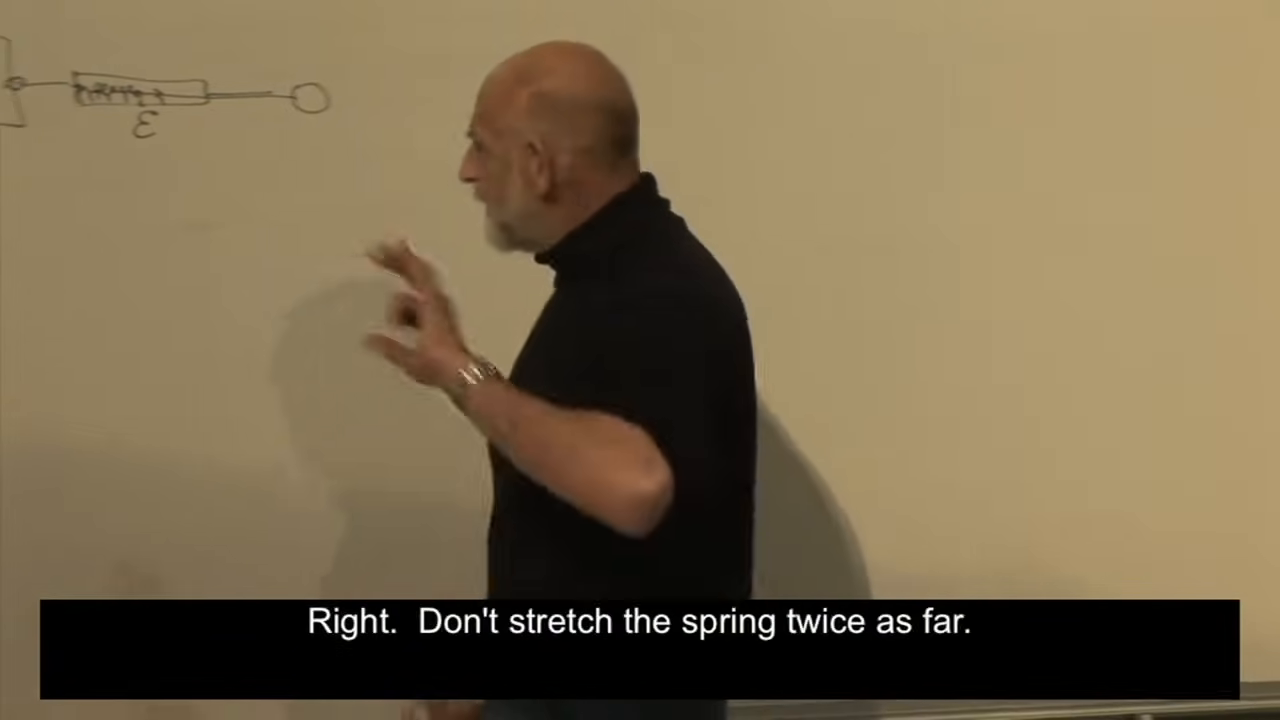
\includegraphics[width=0.84\textwidth]{lecture_02_figure_09.png}
  \caption{用于定义相等的力单位并检验加速度与力成正比的弹簧秤思想实验。}
  \lectureframe{00:22:45}
\end{figure}

这些比较为以下内容提供了经验内容

\begin{equation}
  a\propto F,
  \qquad
  a\propto\frac{1}{m},
  \qquad
  F=ma.
  \label{eq:force-mass-scaling}
\end{equation}

\emph{粒子}一词将用于任何内部结构无关的小物体，而不仅用于基本粒子。

\subsection{为什么仅凭位置不足以构成状态}

我们现在用同样的频闪方法来检验牛顿方程。加速度的中心有限差分为

\begin{equation}
  \ddot x(t)\simeq
  \frac{x(t+\delta)-2x(t)+x(t-\delta)}{\delta^2}.
  \label{eq:second-difference}
\end{equation}

因此牛顿方程意味着

\begin{equation}
  x(t+\delta)
  =2x(t)-x(t-\delta)+\frac{\delta^2}{m}F(t).
  \label{eq:newton-position-update}
\end{equation}

下一个位置不能仅由\(x(t)\)得到。我们还需要前一个位置\(x(t-\delta)\)，或者等价地，当前时刻的速度。起初这使牛顿方程看起来比亚里士多德的方程预测性更差。正确的结论反而是，仅凭位置是对状态的不完整描述。要知道某一时刻所有相关的信息，意味着要知道足以确定后续运动的数据。对于牛顿粒子，这些数据是位置和速度。

\section{动量和相空间}

通过以下方式引入动量

\begin{equation}
  \mathbf p=m\mathbf v=m\dot{\mathbf x}.
  \label{eq:momentum-definition}
\end{equation}

固定牛顿系统的质量被视为常数。一个物体可以失去一块，就像一支笔可以失去笔帽，但那样被描述的物体已经改变了；所选的封闭系统仍然具有恒定的总质量。在\(m\)恒定的情况下，牛顿第二定律变为

\begin{equation}
  \mathbf F=\dot{\mathbf p}.
  \label{eq:newton-momentum-form}
\end{equation}

\begin{figure}[htbp]
  \centering
  \includegraphics[width=0.82\textwidth]{lecture_02_figure_03.png}
  \caption{牛顿定律写成动量的时间导数。}
  \lectureframe{00:32:35}
\end{figure}

对于一个坐标，牛顿运动现在可以写成两个独立状态变量的两个一阶方程：

\begin{align}
  \dot p&=F(x,t),
  \label{eq:first-order-p}\\
  \dot x&=\frac{p}{m}.
  \label{eq:first-order-x}
\end{align}

一个方程说明力如何改变动量；另一个说明动量如何改变位置。它们的一阶离散形式为

\begin{align}
  p(t+\delta)&=p(t)+\delta F(x(t),t)+O(\delta^2),
  \label{eq:momentum-discrete}\\
  x(t+\delta)&=x(t)+\frac{\delta}{m}p(t)+O(\delta^2).
  \label{eq:position-discrete}
\end{align}

给定\(x(t)\)和\(p(t)\)，这些方程确定下一对，然后它成为下一步的输入。轨迹通过重复更新来构建。

\begin{figure}[htbp]
  \centering
  \includegraphics[width=0.84\textwidth]{lecture_02_figure_04.png}
  \caption{两个一阶方程及相应的初始数据。位置和动量共同指定状态。}
  \lectureframe{00:35:47}
\end{figure}

所有对\((x,p)\)构成的空间称为\emph{相空间}。对于一个在三维中运动的粒子，它有六个坐标，

\begin{equation}
  (x,y,z,p_x,p_y,p_z).
  \label{eq:one-particle-phase-space}
\end{equation}

相空间是完全初始条件的空间。位形空间只记录位置；相空间精确地记录运动定律所需的数据。

\begin{classroomqa}
  \audiencequestion{如果力是位置的函数而不是时间的已知函数，更新会变得更复杂吗？\lecturetimestamp{00:36:27--00:37:07}}
  \lecturerresponse{方程仍然具有预测性。一旦\(x\)和\(p\)已知，值\(F(x)\)就已知。方程~\eqref{eq:first-order-p}推进\(p\)，方程~\eqref{eq:first-order-x}推进\(x\)，更新后的对可以再次使用。}
\end{classroomqa}

\section{牛顿弹簧}

回到弹簧，以便两个定律可以在相同的物理基础上进行比较。牛顿给出

\begin{equation}
  m\ddot x=-kx.
  \label{eq:newton-spring}
\end{equation}

暂时设\(m=k=1\)以去除常数。那么

\begin{equation}
  \ddot x=-x.
  \label{eq:normalized-oscillator}
\end{equation}

与指数函数不同，正弦或余弦在两次微分后变回自身的负值。通解可以写成

\begin{align}
  x(t)&=C\cos(t-t_0),
  \label{eq:oscillator-x}\\
  p(t)=\dot x(t)&=-C\sin(t-t_0).
  \label{eq:oscillator-p}
\end{align}

这两个常数承载着两部分初始信息。振幅\(C\)给出最大位移，而\(t_0\)确定相位，这里选取它使得速度在\(t=t_0\)处为零。粒子只在端点处短暂停止。随后它经过原点返回，在那里它的速率和动量最大，并继续振荡。

将式~\eqref{eq:oscillator-x}和\eqref{eq:oscillator-p}平方，得到

\begin{equation}
  x^2+p^2=C^2.
  \label{eq:oscillator-phase-circle}
\end{equation}

因此相空间点在一个半径为\(C\)的圆上运动。不同的初始振幅产生不同的圆；改变\(t_0\)则在同一圆上选择不同的起点。在这些归一化单位下，每个圆都以相同的周期\(2\pi\)被遍历，与振幅无关。

\begin{figure}[htbp]
  \centering
  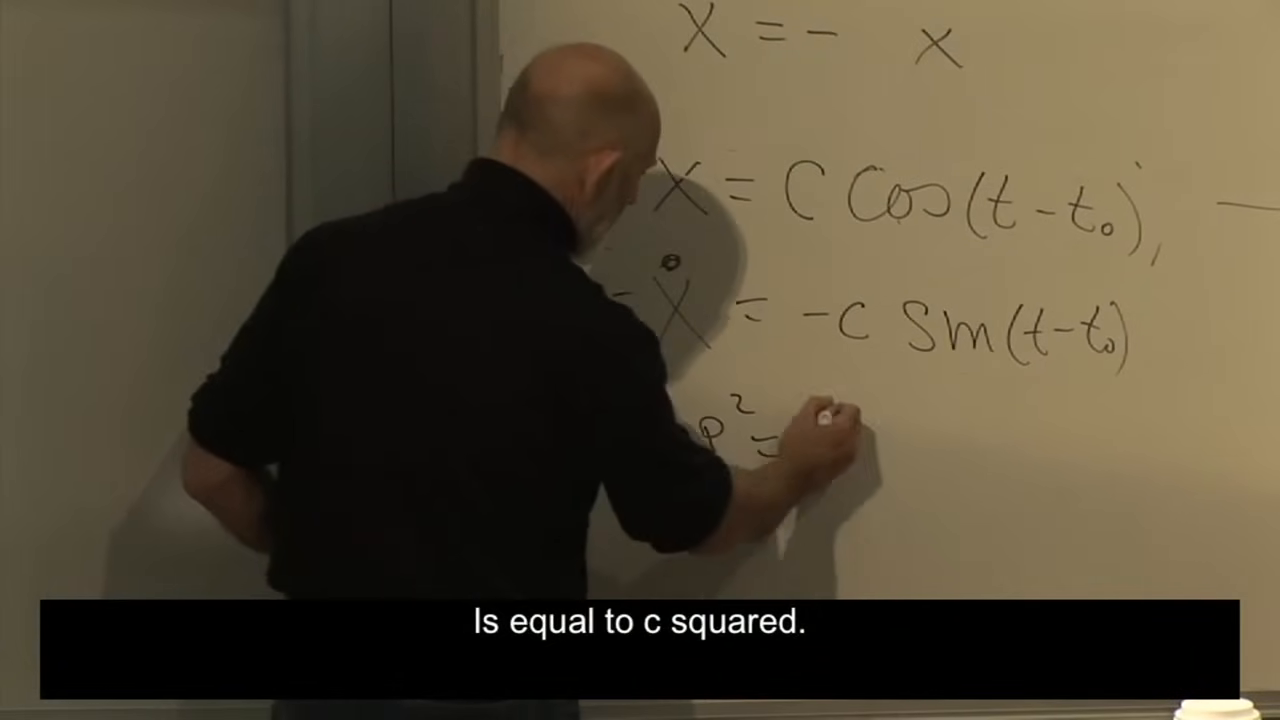
\includegraphics[width=0.84\textwidth]{lecture_02_figure_10.png}
  \caption{振子解及其在\((x,p)\)相平面中的圆轨道。}
  \lectureframe{00:43:20}
\end{figure}

\begin{figure}[htbp]
  \centering
  \begin{tikzpicture}[scale=1.05,>=Latex]
    \draw[->] (-2.6,0) -- (2.75,0) node[right] {$x$};
    \draw[->] (0,-2.4) -- (0,2.55) node[above] {$p$};
    \draw[blue!65!black,thick] (0,0) circle (1.85);
    \draw[->,blue!65!black,thick]
      (1.60,0.93) arc[start angle=30,end angle=72,radius=1.85];
    \fill[red!65!black] (1.60,0.93) circle (2pt);
    \draw[dashed] (0,0) -- (1.60,0.93)
      node[midway,below right] {$C$};
    \node[align=left] at (-1.55,1.85)
      {$x=C\cos(t-t_0)$\\$p=-C\sin(t-t_0)$};
  \end{tikzpicture}
  \caption{相空间轨道同时保留位置和动量。其半径标记运动，而角度随时间均匀推进。}
  \label{fig:oscillator-phase-space}
\end{figure}

投影到水平轴给出\(x\)熟悉的往复运动；投影到竖直轴给出\(p\)的振荡。与亚里士多德式的弹簧不同，不同的圆绝不会彼此坍缩。知道一个相空间点就决定了它的未来和过去。

对于一般的\(m\)和\(k\)，角频率为

\begin{equation}
  \omega=\sqrt{\frac{k}{m}},
  \qquad
  x(t)=C\cos\bigl(\omega(t-t_0)\bigr),
  \label{eq:general-oscillator-frequency}
\end{equation}

而相空间轨道在未缩放的\((x,p)\)平面中变为椭圆。圆形图像是讲座中使用的方便的\(m=k=1\)归一化。

\begin{classroomqa}
  \audiencequestion{如果把振子方程中的二阶导数替换为一阶导数，可预测性会丧失吗？\lecturetimestamp{00:45:23--00:46:04}}
  \lecturerresponse{不会。一阶方程仍然可以从合适的初始数据预测向前的运动。更强的问题是它的流是否足够好地保持区分性从而可逆；相关的普遍定理要等到所需的工具具备后再讨论。}
\end{classroomqa}

\section{时间反演}

振子图像使可逆性变得具体，但也可以对方程进行直接检验。引入反转的时间坐标

\begin{equation}
  T=-t.
  \label{eq:reverse-time}
\end{equation}

那么

\begin{equation}
  \frac{d}{dt}=-\frac{d}{dT},
  \qquad
  \frac{d^2}{dt^2}=\frac{d^2}{dT^2}.
  \label{eq:time-derivative-parity}
\end{equation}

一阶导数在时间反演下改变符号，而二阶导数则不变。因此，自治的亚里士多德方程

\begin{equation}
  m\dot x=F(x)
  \label{eq:aristotle-time-reversal}
\end{equation}

在电影倒放时不保持其形式。一个衰减的弹簧会变成一个自发离开平衡的弹簧。相比之下，

\begin{equation}
  m\ddot x=F(x)
  \label{eq:newton-time-reversal}
\end{equation}

保持不变。反转牛顿式的电影会反转速度但保持加速度不变，因此倒放的电影是另一个允许的解。

\begin{figure}[htbp]
  \centering
  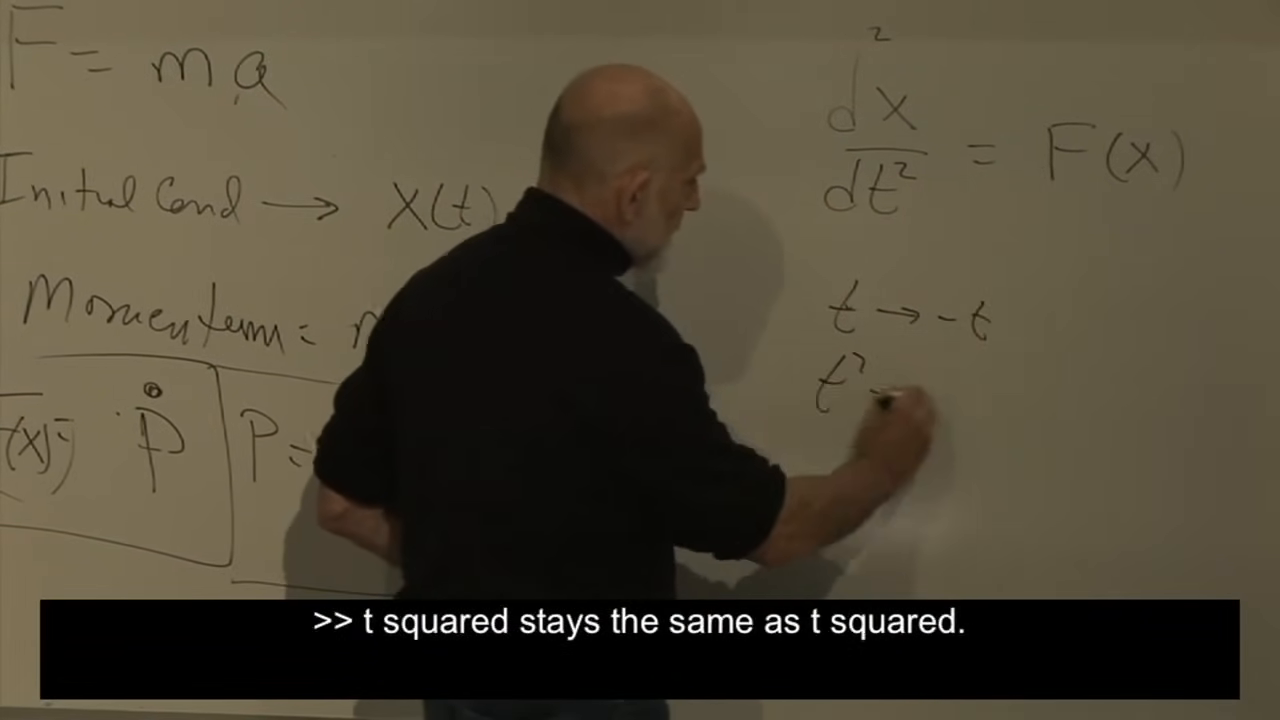
\includegraphics[width=0.84\textwidth]{lecture_02_figure_11.png}
  \caption{在\(t\mapsto -t\)下的板书对比：一阶导数反号，而二阶导数不反号。}
  \lectureframe{00:50:45}
\end{figure}

\begin{classroomqa}
  \audiencequestion{为什么可逆性应当被接受为关于一般物理的前提？\lecturetimestamp{00:46:16--00:48:26}}
  \lecturerresponse{它是被检验的，而不是由定义保证的。我们考察成功的定律，识别共同的实验特征，并将这些特征提升为原理。更深层的逻辑顺序则相反：量子场论更为基本，而牛顿力学通过慢速运动和大质量物体等近似涌现出来。一门课程必须从较简单的定律向上构建，因此现在将可逆性作为一条原理引入，其适用范围将在以后检验。}
\end{classroomqa}

\begin{classroomqa}
  \audiencequestion{可逆性本身是否是牛顿有意识认识到的一个问题？\lecturetimestamp{00:48:28--00:49:02}}
  \lecturerresponse{历史答案并不确定。牛顿当然理解惯性：改变运动状态需要力，而维持匀速运动不需要力。他是否明确地以可逆性来表述这一洞见，则是一个独立的历史问题。}
\end{classroomqa}

\section{循环与守恒量}

相空间圆提示了下一个想法。一条轨迹停留在同一个圆上，绝不会跳到另一个圆上。因此，这个圆可以用一个沿运动保持不变的数来标记。对于归一化振子，这个数是

\begin{equation}
  C^2=x^2+p^2.
  \label{eq:cycle-label}
\end{equation}

差一个二分之一因子，这就是振子的能量。更大的圆具有更大的能量；改变起始相位不会改变它。我们将推导这一陈述，而不是仅仅从图像中读出它，但首先考虑动量。

牛顿第一定律说，不受净力作用的物体以恒定速度运动。它已经包含在第二定律中：

\begin{equation}
  \mathbf F=0
  \quad\Longrightarrow\quad
  \dot{\mathbf p}=0
  \quad\Longrightarrow\quad
  \mathbf v=\text{constant}
  \label{eq:newton-first-from-second}
\end{equation}

对于恒定质量。牛顿第三定律提供了关于粒子间相互作用的真正新信息。

\subsection{大小相等、方向相反且沿连心线的力}

设\(\mathbf F_{ij}\)表示粒子\(j\)施加于粒子\(i\)的力。第三定律中大小相等且方向相反的部分为

\begin{equation}
  \mathbf F_{ij}=-\mathbf F_{ji}.
  \label{eq:newton-third-pair}
\end{equation}

如果这两个力指向同一方向，一个孤立对就可以自发加速。那将是一台仅靠内力产生运动的无推进剂机器。这种行为从未被观察到。

\begin{figure}[htbp]
  \centering
  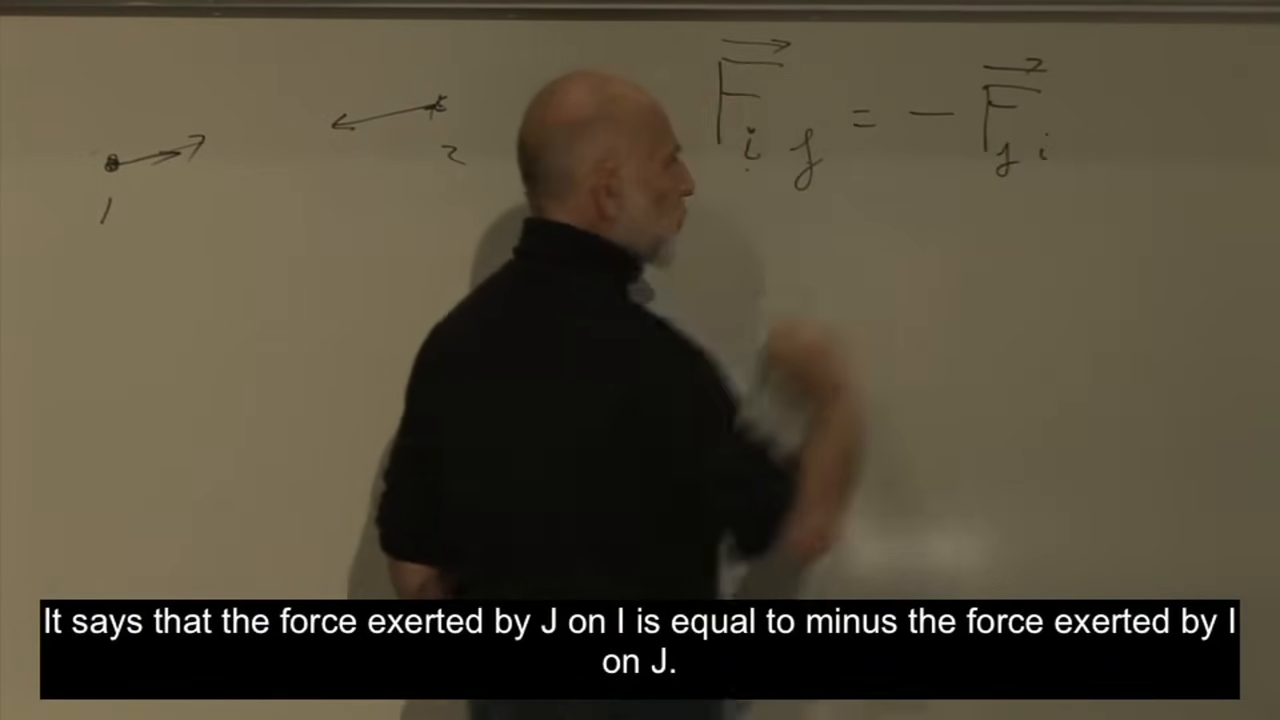
\includegraphics[width=0.84\textwidth]{lecture_02_figure_12.png}
  \caption{相互作用力大小相等且方向相反的带指标表述。}
  \lectureframe{00:59:25}
\end{figure}

对于此处所考虑的点粒子力，这一对力还沿着连接粒子中心的直线作用。大小相等且方向相反但非共线的力可以构成纯力矩，使一个孤立的刚性对转动。连心线力条件排除了这种可能性：

\begin{equation}
  \mathbf F_{ij}\parallel
  (\mathbf r_i-\mathbf r_j).
  \label{eq:central-force-condition}
\end{equation}

大小相等且方向相反的条件将给出线动量守恒。连心线条件与角动量守恒相联系，后者将在以后研究。

\begin{figure}[htbp]
  \centering
  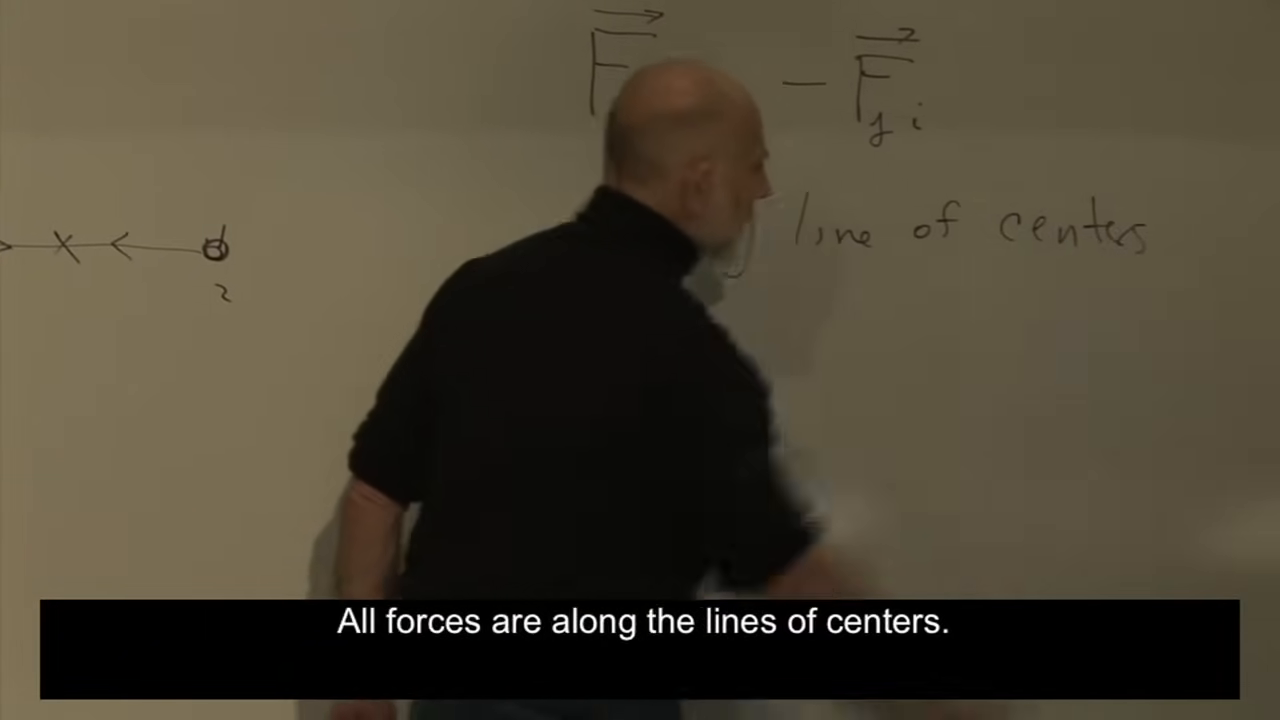
\includegraphics[width=0.84\textwidth]{lecture_02_figure_13.png}
  \caption{牛顿第三定律的连心线力部分：相互作用力沿连接粒子的直线作用。}
  \lectureframe{01:01:38}
\end{figure}

\subsection{总动量}

考虑一个由\(N\)个粒子组成的封闭系统。没有外力；唯一的力是粒子彼此施加的力。力的可加性和牛顿第二定律给出，对每个粒子，

\begin{equation}
  \dot{\mathbf p}_i
  =m_i\ddot{\mathbf r}_i
  =\sum_{\substack{j=1\\j\ne i}}^N \mathbf F_{ij}.
  \label{eq:many-particle-newton}
\end{equation}

将此方程对\(i\)求和：

\begin{align}
  \frac{d}{dt}\sum_{i=1}^N\mathbf p_i
  &=\sum_{i=1}^N
    \sum_{\substack{j=1\\j\ne i}}^N\mathbf F_{ij}
  \notag\\
  &=\sum_{i<j}\bigl(\mathbf F_{ij}+\mathbf F_{ji}\bigr)
  =0.
  \label{eq:momentum-pair-cancellation}
\end{align}

每一次相互作用都出现两次，每个方向各一次，于是这一对相互抵消。定义

\begin{equation}
  \mathbf P_{\mathrm{tot}}=\sum_{i=1}^N\mathbf p_i,
  \label{eq:total-momentum}
\end{equation}

我们得到第一条守恒定律：

\begin{equation}
  \frac{d\mathbf P_{\mathrm{tot}}}{dt}=0.
  \label{eq:momentum-conservation}
\end{equation}

\begin{figure}[htbp]
  \centering
  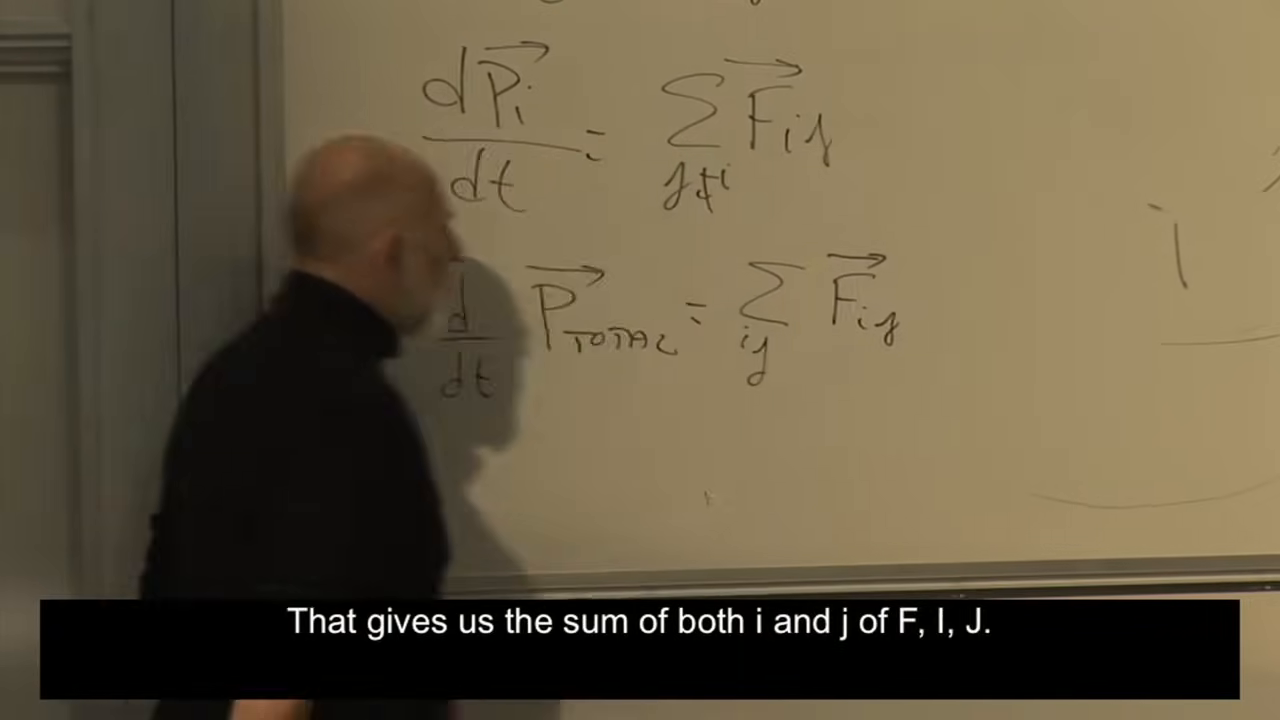
\includegraphics[width=0.84\textwidth]{lecture_02_figure_14.png}
  \caption{对粒子方程求和使成对力相互抵消，从而留下总动量的导数等于零。}
  \lectureframe{01:04:38}
\end{figure}

从历史上看，我们把动量守恒表述为牛顿第三定律的结果。现代物理学往往把动量守恒视为更基本的陈述：如果一个孤立的两粒子系统守恒总动量，其内部动量的变化必须大小相等且方向相反。然而就目前的展开而言，牛顿的路径是有用的那一条。

\section{一维能量}

取一个粒子在一条直线上运动，所受的力只依赖于它的位置：

\begin{equation}
  F=F(x).
  \label{eq:position-force}
\end{equation}

这样的力称为不显含时间的力。这并不意味着运动粒子所感受到的力具有恒定的数值。它的值随\(x(t)\)变化而变化。它的意思是，每当粒子处于同一位置\(x\)时，无论钟表时间如何，它都感受到相同的力。

在一维中，任何足够规则的力函数都可以积分。因此我们通过下式定义势能\(V(x)\)

\begin{equation}
  F(x)=-\frac{dV}{dx},
  \label{eq:potential-definition-1d}
\end{equation}

或等价地

\begin{equation}
  V(x)=-\int^x F(u)\,du+V_0.
  \label{eq:potential-integral}
\end{equation}

相加常数\(V_0\)对力没有影响。把\(V(x)\)想象成\(x\)轴上方一片地形的高度。粒子被推向较低的高度，而斜率越陡的地方力越大。在光滑山丘的顶部或底部，斜率消失，因此那里的力也消失。

\begin{figure}[htbp]
  \centering
  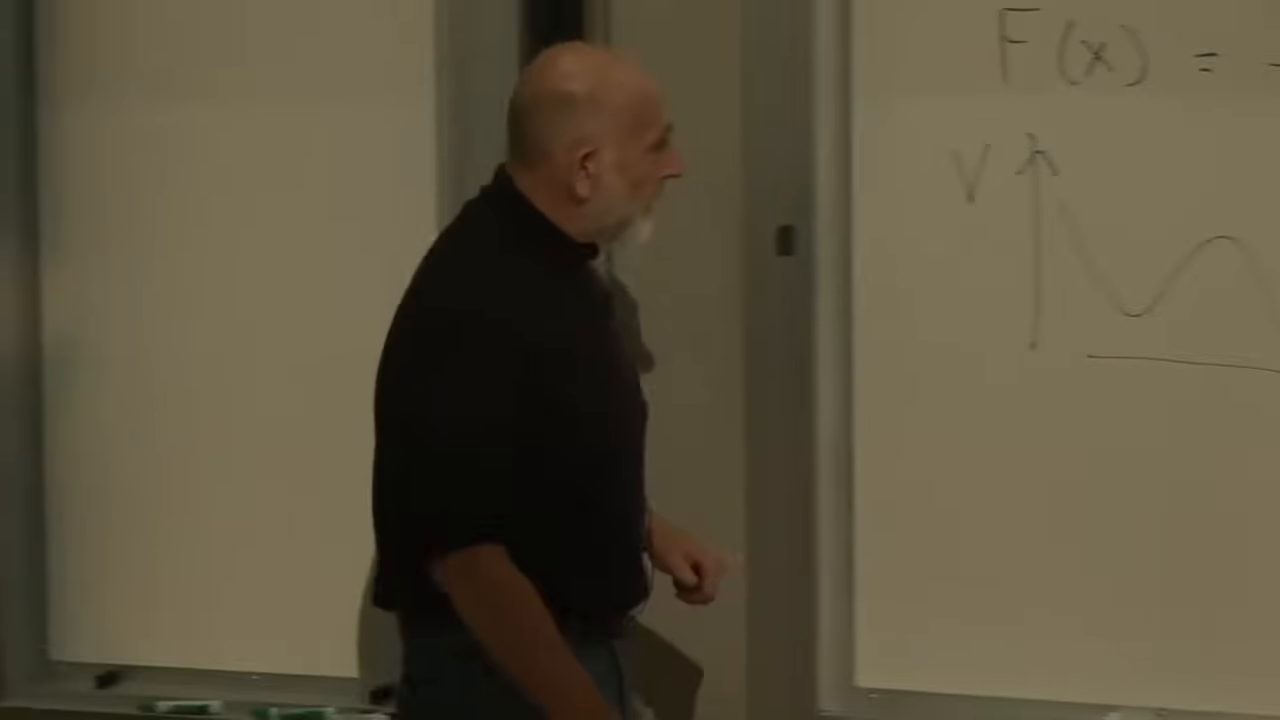
\includegraphics[width=0.84\textwidth]{lecture_02_figure_15.png}
  \caption{势能作为一维地形。力指向下坡方向，其大小由斜率决定。}
  \lectureframe{01:12:57}
\end{figure}

定义动能、势能和总能量为

\begin{equation}
  T=\frac12m\dot x^2,
  \qquad
  E=T+V(x)
  =\frac12m\dot x^2+V(x).
  \label{eq:energy-1d}
\end{equation}

在这个阶段，能量只是赋予这个候选守恒量的名称。它的物理解释由地形提示：向下滚动降低\(V\)，同时增大速率，因而增大\(T\)；向上爬升则相反。牛顿方程证明这种交换是精确的。

对式~\eqref{eq:energy-1d}求导。由于\(m\)是常数，而\(V\)仅通过\(x(t)\)依赖于时间，

\begin{align}
  \frac{dE}{dt}
  &=m\dot x\ddot x+\frac{dV}{dx}\dot x
  \notag\\
  &=\dot x\left(m\ddot x+\frac{dV}{dx}\right).
  \label{eq:energy-derivative-1d}
\end{align}

牛顿定律和\(V\)的定义给出

\begin{equation}
  m\ddot x=F=-\frac{dV}{dx}.
  \label{eq:newton-potential-1d}
\end{equation}

因此式~\eqref{eq:energy-derivative-1d}中的括号项消失：

\begin{equation}
  \frac{dE}{dt}=0.
  \label{eq:energy-conservation-1d}
\end{equation}

\begin{figure}[htbp]
  \centering
  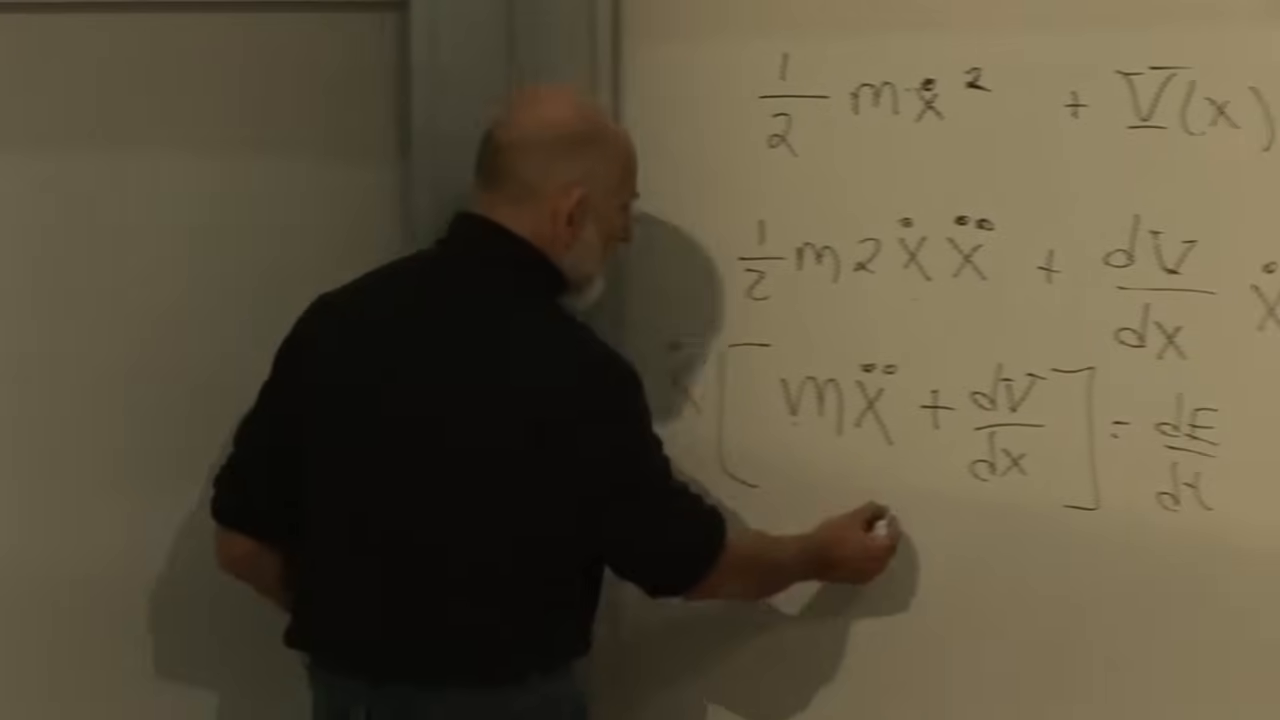
\includegraphics[width=0.84\textwidth]{lecture_02_figure_16.png}
  \caption{一维能量导数被分解为速度乘以牛顿方程。}
  \lectureframe{01:19:18}
\end{figure}

在一维中，除了一个规则的依赖于位置的力之外，不需要额外的动力学假设，因为每一个这样的力都容许一个原函数。

\section{多维情形与保守力}

对于一个坐标为\(x_i\)的粒子，牛顿方程的分量形式为

\begin{equation}
  F_i(\mathbf x)=m\ddot x_i.
  \label{eq:newton-components}
\end{equation}

力的分量\(F_i\)可以依赖于所有坐标，而不只是\(x_i\)。我们希望找到一个标量函数\(V(\mathbf x)\)，使得

\begin{equation}
  F_i(\mathbf x)
  =-\frac{\partial V(\mathbf x)}{\partial x_i},
  \qquad
  \mathbf F=-\boldsymbol\nabla V.
  \label{eq:gradient-force}
\end{equation}

与一维构造不同，这一点并非自动成立。三个任意函数\(F_1,F_2,F_3\)通常包含比一个标量函数的导数更多的独立信息。等价地说，只有当力场满足相容性条件，例如相应的混合偏导数相等时，势才存在；在单连通区域中，这由\(\boldsymbol\nabla\times\mathbf F=0\)表示。
因此，我们把式~\eqref{eq:gradient-force}视为对所考虑的这一类力的物理公设，而不是数学恒等式。

\begin{figure}[htbp]
  \centering
  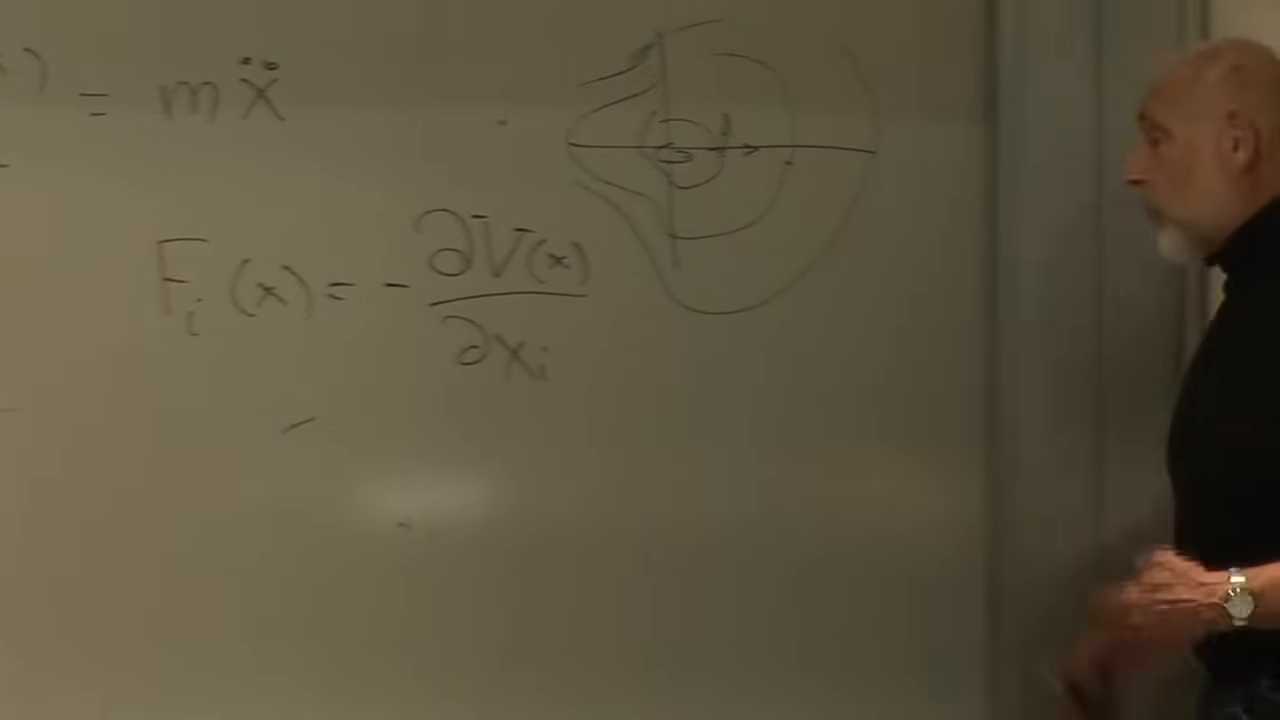
\includegraphics[width=0.84\textwidth]{lecture_02_figure_17.png}
  \caption{多维力律与势的等值线草图。力穿过等值线指向\(V\)减小的方向。}
  \lectureframe{01:24:15}
\end{figure}

在等值线图上，\(V\)沿每条等值线为常数。梯度垂直于这些曲线并指向最陡上升方向；力\(-\boldsymbol\nabla V\)指向最陡下降方向。

\begin{figure}[htbp]
  \centering
  \begin{tikzpicture}[scale=1.0,>=Latex]
    \draw[->] (-3.0,0) -- (3.1,0) node[right] {$x_1$};
    \draw[->] (0,-2.4) -- (0,2.55) node[above] {$x_2$};
    \draw[orange!65!black,thick]
      plot[smooth cycle] coordinates
      {(-0.55,-0.35) (0.15,-0.55) (0.72,-0.10) (0.50,0.53) (-0.25,0.65)};
    \draw[orange!65!black,thick]
      plot[smooth cycle] coordinates
      {(-1.15,-0.75) (0.20,-1.10) (1.35,-0.25) (1.10,0.95) (-0.45,1.25)};
    \draw[orange!65!black,thick]
      plot[smooth cycle] coordinates
      {(-1.85,-1.20) (0.15,-1.70) (2.15,-0.40) (1.70,1.50) (-0.80,1.85)};
    \draw[->,blue!65!black,very thick] (1.62,0.73) -- (0.82,0.20)
      node[midway,above left] {$\mathbf F$};
    \draw[dashed,->,red!65!black,thick] (0.82,0.20) -- (1.62,0.73)
      node[midway,below right] {$\boldsymbol\nabla V$};
    \node[orange!65!black] at (-1.62,1.45) {$V=V_3$};
    \node[orange!65!black] at (-0.92,0.92) {$V=V_2$};
    \node[orange!65!black] at (-0.35,0.30) {$V=V_1$};
  \end{tikzpicture}
  \caption{标量势的等值线。梯度垂直于等值线，而保守力指向相反方向。}
  \label{fig:potential-contours}
\end{figure}

当式~\eqref{eq:gradient-force}成立时，定义

\begin{equation}
  E=\frac12m\sum_i\dot x_i^2+V(x_1,\ldots,x_n).
  \label{eq:energy-many-coordinates}
\end{equation}

动能项是质量的一半乘以速度矢量长度的平方。求导并应用多变量链式法则得到

\begin{align}
  \frac{dE}{dt}
  &=m\sum_i\dot x_i\ddot x_i
    +\sum_i\frac{\partial V}{\partial x_i}\dot x_i
  \notag\\
  &=\sum_i\dot x_i
    \left(m\ddot x_i+\frac{\partial V}{\partial x_i}\right)
  =0.
  \label{eq:energy-derivative-multidimensional}
\end{align}

这个证明正是带上了指标的一维证明，但其前提更强：力的各分量必须全部来自同一个势。

\begin{figure}[htbp]
  \centering
  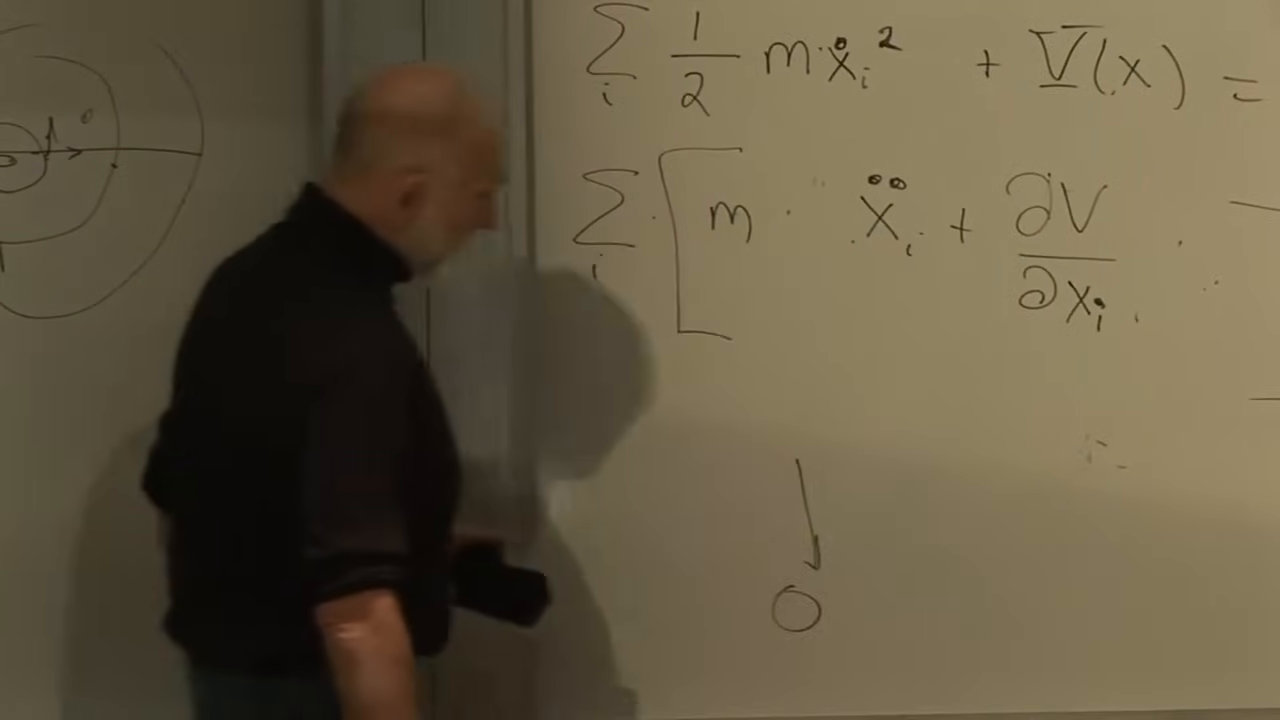
\includegraphics[width=0.84\textwidth]{lecture_02_figure_18.png}
  \caption{带指标的能量导数。每个括号都因牛顿方程的相应分量而为零。}
  \lectureframe{01:28:30}
\end{figure}

对于三维空间中的\(N\)个粒子，将所有坐标收集到一个列表中

\begin{equation}
  \begin{aligned}
    q_a={}&(x_1,y_1,z_1,x_2,y_2,z_2,\ldots,\\[-0.2em]
           &\phantom{(}x_N,y_N,z_N),\\
    &a=1,\ldots,3N.
  \end{aligned}
  \label{eq:flattened-coordinates}
\end{equation}

共有\(3N\)个坐标条目，但只有\(N\)个粒子质量；同一个质量出现在属于给定粒子的三个条目中。如果

\begin{equation}
  F_a=-\frac{\partial V(q_1,\ldots,q_{3N})}{\partial q_a},
  \label{eq:many-particle-conservative-force}
\end{equation}

那么

\begin{equation}
  E=\sum_{A=1}^{N}\frac12m_A\lvert\dot{\mathbf r}_A\rvert^2
    +V(\mathbf r_1,\ldots,\mathbf r_N)
  \label{eq:many-particle-energy}
\end{equation}

由同样的计算可知其守恒。由势产生的力被称为\emph{保守}力，正是因为它们支持这一守恒定律；这个形容词没有任何政治含义。

\section{作为能量等值线的振子}
\enlargethispage{3\baselineskip}

对于弹簧力\(F=-kx\)，式~\eqref{eq:potential-definition-1d}给出

\begin{equation}
  V(x)=\frac12kx^2+V_0.
  \label{eq:spring-potential}
\end{equation}

选取\(V_0=0\)，振子能量为

\begin{equation}
  E=\frac12m\dot x^2+\frac12kx^2
   =\frac{p^2}{2m}+\frac12kx^2.
  \label{eq:oscillator-energy}
\end{equation}

对于\(m=k=1\)，

\begin{equation}
  2E=p^2+x^2=C^2.
  \label{eq:oscillator-energy-circle}
\end{equation}

因此，先前发现的相空间圆就是等能线。对于更一般的一维势，等值线不必是圆，但运动仍然位于曲线上

\begin{equation}
  \frac{p^2}{2m}+V(x)=E
  \label{eq:general-energy-contour}
\end{equation}

在\((x,p)\)平面中。这把我们带回到第一讲的想法：当轨迹保持在不同的循环或轨道上时，一个数可以标记这些轨道并在整个运动过程中保持不变。

现在我们已经有了状态空间、牛顿更新方程以及前两条守恒定律。力学的下一个表述将从最小作用量原理出发，并导向拉格朗日量、哈密顿量、角动量，以及这些例子背后更一般的结构。

\begin{classroomqa}
  \audiencequestion{分发的讲义与黑板上的内容对应得有多紧密，图在哪里？\lecturetimestamp{01:37:56--01:38:54}}
  \lecturerresponse{讲义应当紧跟讲课内容；如果黑板上的材料缺失，可能是发错了文件。图还没有准备好；他开玩笑说，等继续教育项目支付下一张支票时它们就会出现。}
\end{classroomqa}